\chapter{Introduction}
\label{chap:introduction}
\addcontentsline{toc}{chapter}{Introduction}
\section{Human population and the need for improved agriculture}
By 2019 the human population has reached 7.7 billion and this number will continue to increase by 2 billion each year.
According to United nations the human population will reach 9.7 billion by 2050,
although this projection is not uniform with fertility rates going down in some regions of the world while increasing in others. \cite{population_2019}
For instance, India is predicted to surpass China and be the highest populated country by 2027. This growing population will require more food and land resources.\cite{population_2019}
%We also need to realize that there is a segregation based on availability.
But for a sustainable development, land resources need to be utilised judicially.
The amount of cultivable land is not increasing as such. In fact there is only an approximate 5\% increase in cultivable land in developed countries in the coming years although the inflation in population is far more profound.\cite{fao_agri} 
On the other hand another bigger issue is approximately one-third of all the food produces get wasted before consumption which is about 1.3 billion tons per year. \cite{fao_food_loss}
Hence, food resources can be increased with better and improved agricultural practices. 
Currently even with the use of pesticides the amount of crops destroyed by bacteria, fungi and
pests is a considerable amount and as the temperature increases due to global warming the problem of 
microorganisms and pests is going to escalate too.\cite{Gurr2013} 
So to tackle this issue, pharmaceuticals have to come up with better and improved antibiotics, fungicides and pesticides. In the following sections we will discuss more about some of the challenges in developing new 
antibiotics.

\section{History and discovery of fungicides}
Plants have suffered from various diseases since they started growing on this planet.
In the initial days of agriculture humans couldn't quite fathom that plants like humans
are vulnerable to diseases. Insects can be seen and can be distinguished in order to be kept off from plants if they have been observed to be detrimental to plants.\cite{russell2005} But pathogens and microorganisms being of microscopic size, were harder and more difficult to detect. In ancient India, around 500AD people used various herbs if the plant was seen to be suffering from some disease. These ad-hoc treatments persisted for a while till the nineteenth century when the pathogens that afflicted humans were discovered. There was no evident industry dedicated to the development of medicines to treat plant diseases. But as the in the later half of nineteenth century, chemical industry emerged, inorganic salts like copper sulphate was used as a treatment for certain fungal diseases in plants.\cite{russell2005} By the 1900s various specific disciplines were dedicated towards the study of plant diseases and the early medicines for them were phenyl mercury acetate, mercurous chloride, copper oxide and so on. Soon they were found to be injurious to the environment, affecting ground water and harmful to animals exposed to these chemicals . In addition to this, by the 1960s various fungus responsible for plant diseases had started showing resistance towards the chemical fungicides. This lead to the development and discovery of pesticides and fungicides of biological origin. \cite{russell2005} Currently one such product available in the market is Serenade \textsuperscript{\textregistered} Opti from Bayer. But further research needs to be conducted to come up with more novel biofungicides after taken into consideration the various ecological and public health responsibilities.\cite{Avis2016}

\section{Antibiotics: Pros and Cons}
Antibiotics have been used by mankind for their own consumption since 300-350BC. Evidence of which has been found in the 
human remains from that era and even in the Roman period too. \cite{Armelagos2010, 
Villanueva1980, Anderson1989} 
Even before western medicine caught up to antibiotics, traditional forms 
of medicine that were essentially antibiotics have always been present 
in various cultures.\cite{Aminov2010} The most famous example of this is 
the discovery of  artemisinin also known as 'qinghaosu' in china where 
this has been used as a medicine for hundreds of years. Artemesinin was 
extracted from  Artemisia plants in 1970 as a potent antimalarial 
drug.\cite{Su2009}

The modern antibiotic era started with Paul Ehrlich and Alexander Fleming. 
Ehrlich observed that certain dyes like aniline, stain only certain bacteria and not all. 
From this he concluded that targeted chemical compounds can be found that 
kills only disease causing organism and not the healthy cells. 
Their target disease was syphilis which was endemic at that time and a need for less drastic medication
was necessary. Thus the scientists tested syphilis against hundreds of 
compunds which in   modern drug discovery terms we call high-thoroughput screening, before they stumbled upon 
Neosalvarsan.\cite{Hata1910}
Soon after this came the era of antibiotics where different chemical compound classes were 
found which were effective against various bacteria and fungi, most famous among them is penicillin which is effective against a broad spectrum of bacteria.\cite{Fleming1929}
But these drugs come with a huge price. Microorganisms can develop resistance towards 
these compounds quickly. In fact we now have evolved microorganisms called "super bugs" that 
are resistant to most antibiotics. Each year thousands of patients die in 
hospitals in developed countries as they are exposed to these highly resistant species of 
bacteria that are fatal for immune compromised patients like children and elderly in the hospitals. The reason behind the evolution of \"smart\" bacteria is simple, bacteria have existed in this world way longer than humans and they can come up with 
mutations in their genetic code to adapt to a hostile environment. So although we humans 
can develop drugs there will always be this constant race of finding drugs which can become
obsolete due to resistance from pathogens. \cite{Davies2010} 
Currently the pharmaceutical industry spends 10 million dollars to get one drug into market and it takes \~ 10 years of work by thousands of people. Hence the 
increasing need to come up with antibiotics with broad spectrum of effectiveness.
%%%%%Add citation%%%%%


\section{Bio-control agents}
Instead of using chemicals to treat plant diseases different government agencies have been pushing for environmental friendly, biologically derived molecules as pesticides, fungicides and bactericide.
Sometimes microorganisms secrete certain molecules
that can kill other organisms compete for the same food resources. 
These microorganisms are called bio-control agents.\cite{Wilson2009}
Recently these have been used for post-harvest control of diseases in 
potatoes, tomatoes and fruits. 
Currently 14 bacteria and 12 fungi are used as bio-control agents and 
commercially available.\cite{Fravel2005}
The main mechanism that these microorganisms use to kill pathogens are 
antibiosis. So the antagonists secrete some low molecular weight 
antibiotics that can inhibit the growth of the 
pathogen.\cite{Lynch2005}

Other methods that these organisms use for bio-control are stimulating the plant's own defense mechanism which renders the host body more resistance towards harmful bacterial and fungal attacks. This is called induced systematic resistance.
This is seen in several \textit{Pseudomonas} and \textit{Serratia} species of bacteria.\cite{Aziz2009,Monica2009,Mantil2018}
This method is so effective that plants treated with these microorganisms in the roots render protection in the above soil parts of the same.\cite{Thonart2007}
In the following discussion we will discuss one of the chemicals secreted by these bio-control agents which kill the pathogens directly.

\section{Antimicrobial peptides}
Antimicrobial peptides(AMP) were first obtained from purifying one of the bacterial species of \textit{Bacillus} genus in 1939.\cite{Dubos1939,Ren2013}
These are one of the bio-control agents targeted by pharmaceutical companies 
when faced with antibiotic resistance from different small molecules.
The first animal derived antimicrobial peptides were discovered in rabbit leukocytes in 1956 and finally they were also discovered in human leukocytes.\cite{Hirsch1956,Spitznagel1963,Ren2013}

In animals, AMPs are usually found in tissues most exposed for any attacks from pathogens. So they are usually the first line of defense for the body's immune system. Till now thousands of AMPs have been discovered or synthesized. They are found in prokaryotes and eukaryotes
and they come in all 3D shapes \textit{\--} $\alpha$-helix,$\beta$-sheets and loops. They can be cyclic and even change shape when they are close to their targets.\cite{LEIPPE1999,Jabra2010,Huang2010,Sonnevend1970}
Usually the antimicrobial peptides attack the cell membrane of the pathogens instead of binding to specific proteins like conventional antibiotics.\cite{Hancock2006} They cause leakage in the cell membrane which lead to the death of the microorganisms.
Because of their unconventional target and selectivity towards cell wall/membrane, it is hard for the pathogen to change the composition of their cell membrane and thus hard to develop resistance against these peptides.\cite{Hancock2006,Ren2013} They are fast acting and hence can kill the pathogens in seconds.\cite{Fischetti2001} 
Although there are several advantages of developing AMPs as the next class of antibiotics, AMPs have a long way to go before they are pushed further as leads in drug targets. The reasons being their toxicity to humans, susceptibility to proteases, high production costs, lack of selectivity in some cases and peptide folding problems.\cite{Tossi2002}

\section{Fengycin: Fungicidal Lipopeptides}
Fengycin is a family lipopeptide secreted by \textit{Bacillus subtilis}
as a response against fungal attacks. 
It was first isolated from the bacteria in 1986 by Vanittanakom et al.\cite{Vanittanakom1986}
They also found that fengycins were not effective against bacteria and showed low blood toxicity(hemolysis).\cite{Vanittanakom1986}
Fengycin like other AMPs attack the cell membrane to cause leakage It is highly specific to fungal cells and have been found to be a component of Serenade \textsuperscript{\textregistered} (Bayer).
Apart from this method fengycin elicit induced systematic resistance in
plants. This is one of the main reasons why \textit{Bacillus subtilis} shares a symbiotic relationship with various plants. 
Recently, Piewngam et al also found that fengycins can be used as a quorum sensor blocker for eradication of \textit{Staphylococcus aureus} from human gut.\cite{Otto2018}
This proved that consumption of \"good bacteria\" can indeed improve human health.
The structure of fengycin is quite fascinating. As shown in figure \ref{fig:ch2_chemical_str} fengycin is ten-amino acids long with a 15-17 long acyl chain. Out of ten residues, eight form a lactone ring between Tyr-3 and the C-terminus of the molecule. The cyclization and short hydrophobic hydrocarbons are central features in all the lipopeptides synthesized by \textit{Bacillus subtilis} like surfactins and iturins. \cite{Jacques2007} Fengycins are synthesized via non-ribosomal pathway by the bacteria
which has lead to the presence of D-amino acids in their composition and the closing of the peptide ring via ester formation. \cite{Jacques1999}
\begin{figure}
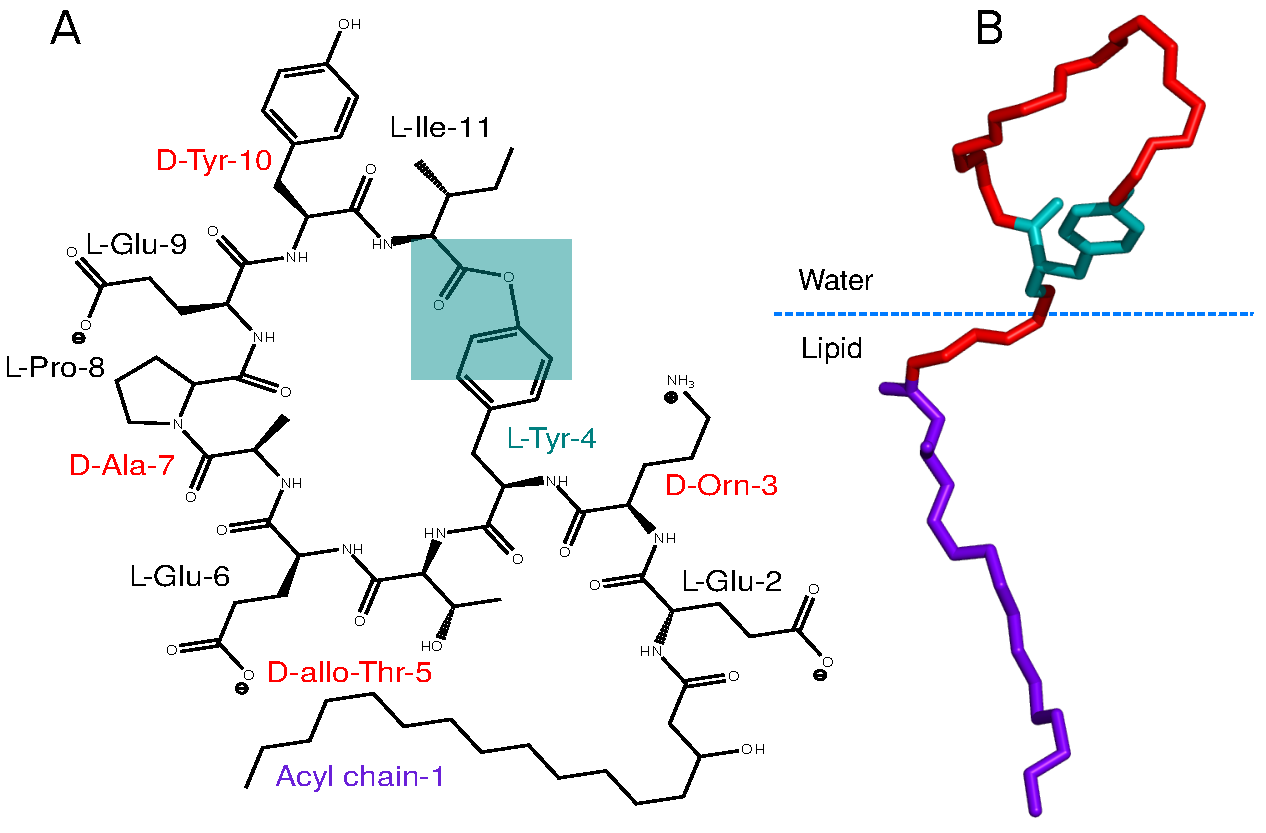
\includegraphics[width=0.9\textwidth]{chapter2_figs/structure.pdf}
\caption{\label{fig:ch2_chemical_str} (A) Chemical
structure of fengycin(Adapted from Horn et al).\cite{Liu2007,HornGrossfield2013};
 (B) 3D orientation of one of the
conformations of fengycin during our simulation.
Violet sticks represent the acyl tail, red sticks
show the peptide backbone and cyan sticks stand for
the C-terminus and Tyr-4 ester linkage.}
\end{figure}

In my thesis I have looked at the lipid-fengycin and fengycin-fengycin interactions that lead to cell leakage. This can be leveraged to design highly specific target based peptide drugs.
In the following section I have discussed some of the aspects of cell membrane which is the target for fengycins to lay the ground for my thesis project.

\section{Cell membranes: evolution and characteristics}
Cell is the unit of life and the cell membrane is the boundary that separates the 
cell from the environment. Without the cell membrane a cell cannot claim its 
existence. Apart from this function cell membrane is also responsible for 
communication, transport and certain metabolic activities. Currently, the structure of cell 
membrane is based on the fluid mosaic model as shown in figure \ref{fig:fluid_mosaic}.\cite{Nicholson1972}
%%%%Add the figures made on keynote
%%%% Dont know why this figure wont be here
\begin{figure}
   \label{fig:fluid_mosaic}
   \centering
   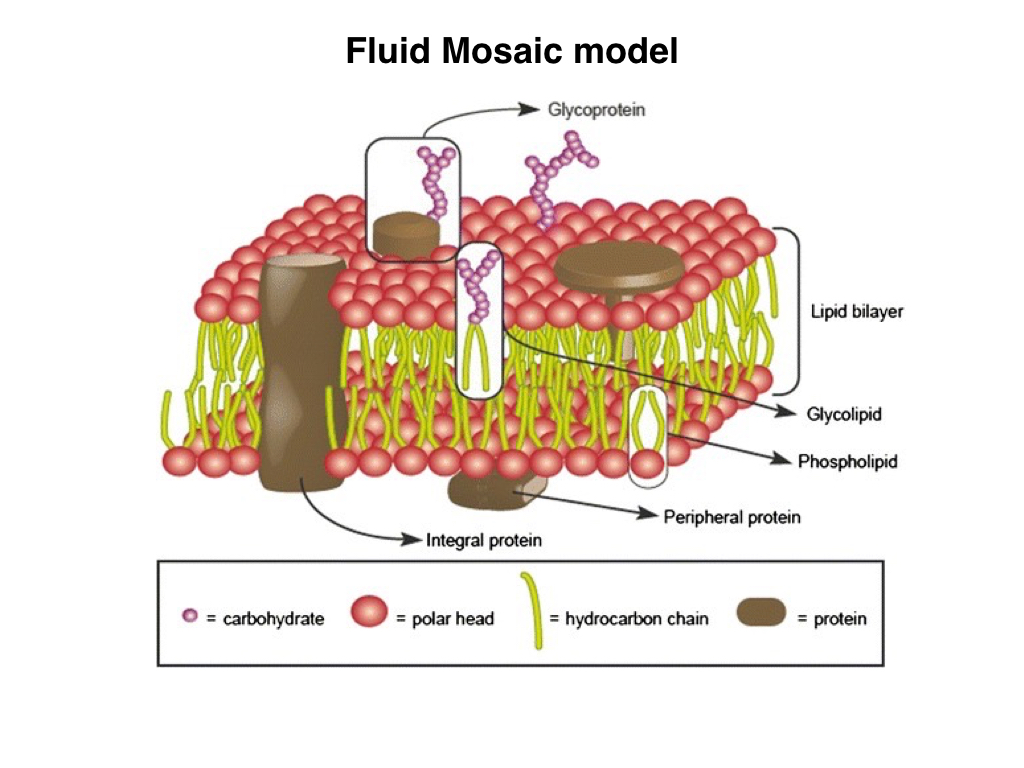
\includegraphics[width=0.9\textwidth]{chapter1_figs/fluid_mosaic_model.jpeg}
   \caption{Fluid mosaic model \cite{Lombard2014}}
\end{figure}
In order to understand the mechanism of fengycin, it is also important 
to discuss the complexities of the cell membranes which these 
molecules are targeting. 
The membranes consists of molecules which are amphiphilic constituting hydrophobic and 
hydrophilic parts mostly glycoproteins, integral proteins and lipids. Lipids constitute 
the highest proportion in membranes. Due to the amphiphilic nature of lipids, 
eukaryotic membranes are bilayers with the hydrophilic parts of lipids face aqueous 
environment in the extracellular and intracellular part and the hydrophobic interior 
remains in the interior of the membrane as shown in figure%%add the figure
. \cite{vonHippe1974,Lombard2014}
Integral proteins are the proteins which are embedded in the membranes and also consist 
of hydrophilic and hydrophobic components. There is also another type of proteins found 
partly bound to membranes called peripheral proteins. The term "fluid" is used for membranes because all these components of the membrane can diffuse laterally along the membrane while the the term "mosaic" refers to the diversity of different molecules that comprise the membrane.\cite{Lombard2014}
The composition of the membrane varies with different classes of organisms for instance bacteria, fungi and mammals have different phospholipids constituting their respective membranes. \cite{Walker2010}.

For around 450 million years bacteria has been on this earth. \cite{bacteriaevol}
In order to survive this world for so long, bacteria needed to have extra protection.
Bacterial cell envelope is very complex although it is one of the earliest inhabitants
of the world. Depending on the outer envelope composition there are two types of bacteria:
Gram positive and gram negative depending on whether it absorbs a particular stain made by Christian George in 1884.
It consists of outer membrane mainly made up of glycolipids. Gram negative bacteria like E.Coli has the outer membrane while the Gram positive ones don't.\cite{Walker2010}
The next layer in the bacterial cell envelope is the peptidoglycan. This is the layer which absorbs 
a particular stain by George Gram so that the bacteria could be classified into 
gram positive and negative bacteria. Bacillus subtilis is a gram positive bacteria and it secretes fengycin, surfactin and iturins.
The last layer in the membrane consists of mainly phospholipids, phosphatidyl ethanolamine and phosphatidyl glycerol which
is negatively charged.
 Fungus have both a cell wall and a cell membrane. The cell membrane consists of 
sphingolipids, ergosterol and phospholipids mainly phosphatidyl ethanolamine and
phosphatidylcholine.\cite{deshpande2016}
Mammals, on the other hand, have phospholipids, sphingolipids and cholesterol. \cite{Kroon2011}
\begin{figure}
\label{fig:phospholipids}
    \centering
    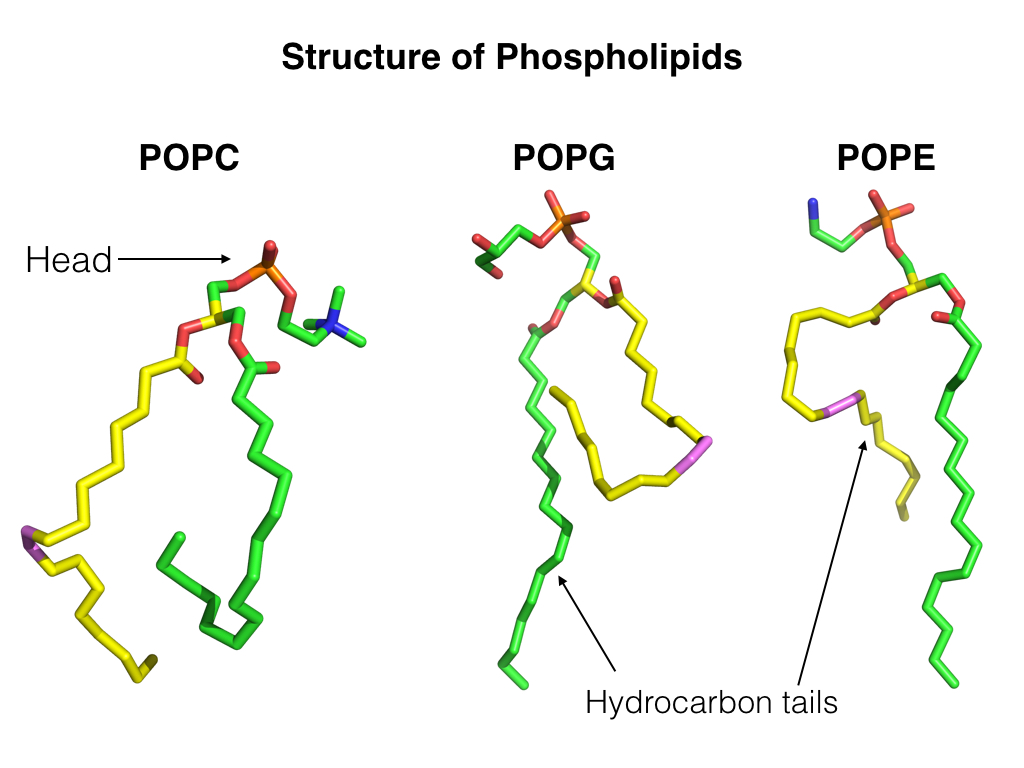
\includegraphics[width=0.6\textwidth]{chapter1_figs/phospholipids.jpeg}
    \caption{Phospholipids}
    \label{fig:phospholipids}
\end{figure}{}

Phospholipids have two long hydrocarbon chains which form the hydrophobic core while the 
phosphate group forms the hydrophilic head as shown in figure \ref{fig:phospholipids}. \cite{Slotte2002}
Apart from the glycerol based phospholipids there is also 
sphingolipids based ones in mammals. The main phospholipid is 
phosphotatidyl choline in the mammals. \cite{Kroon2011,Slotte2002}
Around 15 years ago through electron micropscopy scientists found that phopholipids along with cholesterol 
accumulate and form a separate phase in the membranes.\cite{Kroon2011} This is
the liquid ordered phase(L$_O$)
Due to this inherent ordering properties of cholesterol 
mammalian cell membranes have different properties than 
fungal and bacterial membranes.
All these properties of the membrane along with the different structures of the phospholipid headgroups are important as we look into the membrane-fengycin interactions.

%%%%Revision needed here
%%%%Make a figure with cholesterol ergosterol phospholipids PE/PC/PG

\section{Molecular dynamics simulations}
\label{ss:mdsim}
Molecular dynamics simulations simply means 
we are imitating the motion of molecules taking into 
consideration various physical laws. In this section I will point out some of the motivations to use 
this method to study fengycins.

Membrane proteins are hard to isolate because their structure is 
dependent on the environment in which they are. So to maintain the 
hydrophobic interior of lipids, membrane proteins are usually isolated 
using detergents to emulate the amphiphilic nature of lipids. 
Then X-ray crystallography or solid state NMR is conducted to isolate the structure
of the protein.This is an extensive process and the yield of purified protein may
be too low to get good results. Thus different MD simulations are conducted 
in the presence of lipids to isolate the structure-function relationship of the membrane protein.
In case of fengycins there is an additional issue. Fengycins
come in different mutants with the variation
being single or double points.
Thus it is hard to isolate a single sequence of fengycins.
Since 
molecular dynamics simulations uses computational resources it is much 
easier to build and manipulate the structure of fengycins.
%Molecular dynamics simulations are useful when 
%%we don't have high resolution data for the process 
%or high cost to evaluate the process.
%In drug discovery projects, simulations are done with the target and
%the ligand to see whether ligand will fit into the binding pocket, calculate binding affinity and calculation of off rates of the ligand.
%and thus confirming whether synthesizing of the molecule is a good
%investment both in terms of monetary and time.
Molecular dynamics can be considered as a real time microscope
where we can have highest possible resolution with the changes occuring 
in the femtosecond timescale. 
In these simulations we first build a system which is comprised of atoms. 
We have all the coordinates of the atoms in the system. Then we define 
the forces acting on the system due to bonds between the atoms, angles 
made by the bonds and the dihedral angles due to the inherent nature of 
the chemical species. These contribute to the forces acting on the atoms.
The atoms follow the Newton's equations of motions and we use that to 
determine the way these molecules move with time.
Based on the velocities and positions of these molecules we can predict 
the macroscopic properties of the system. 

\begin{figure}
%\centering
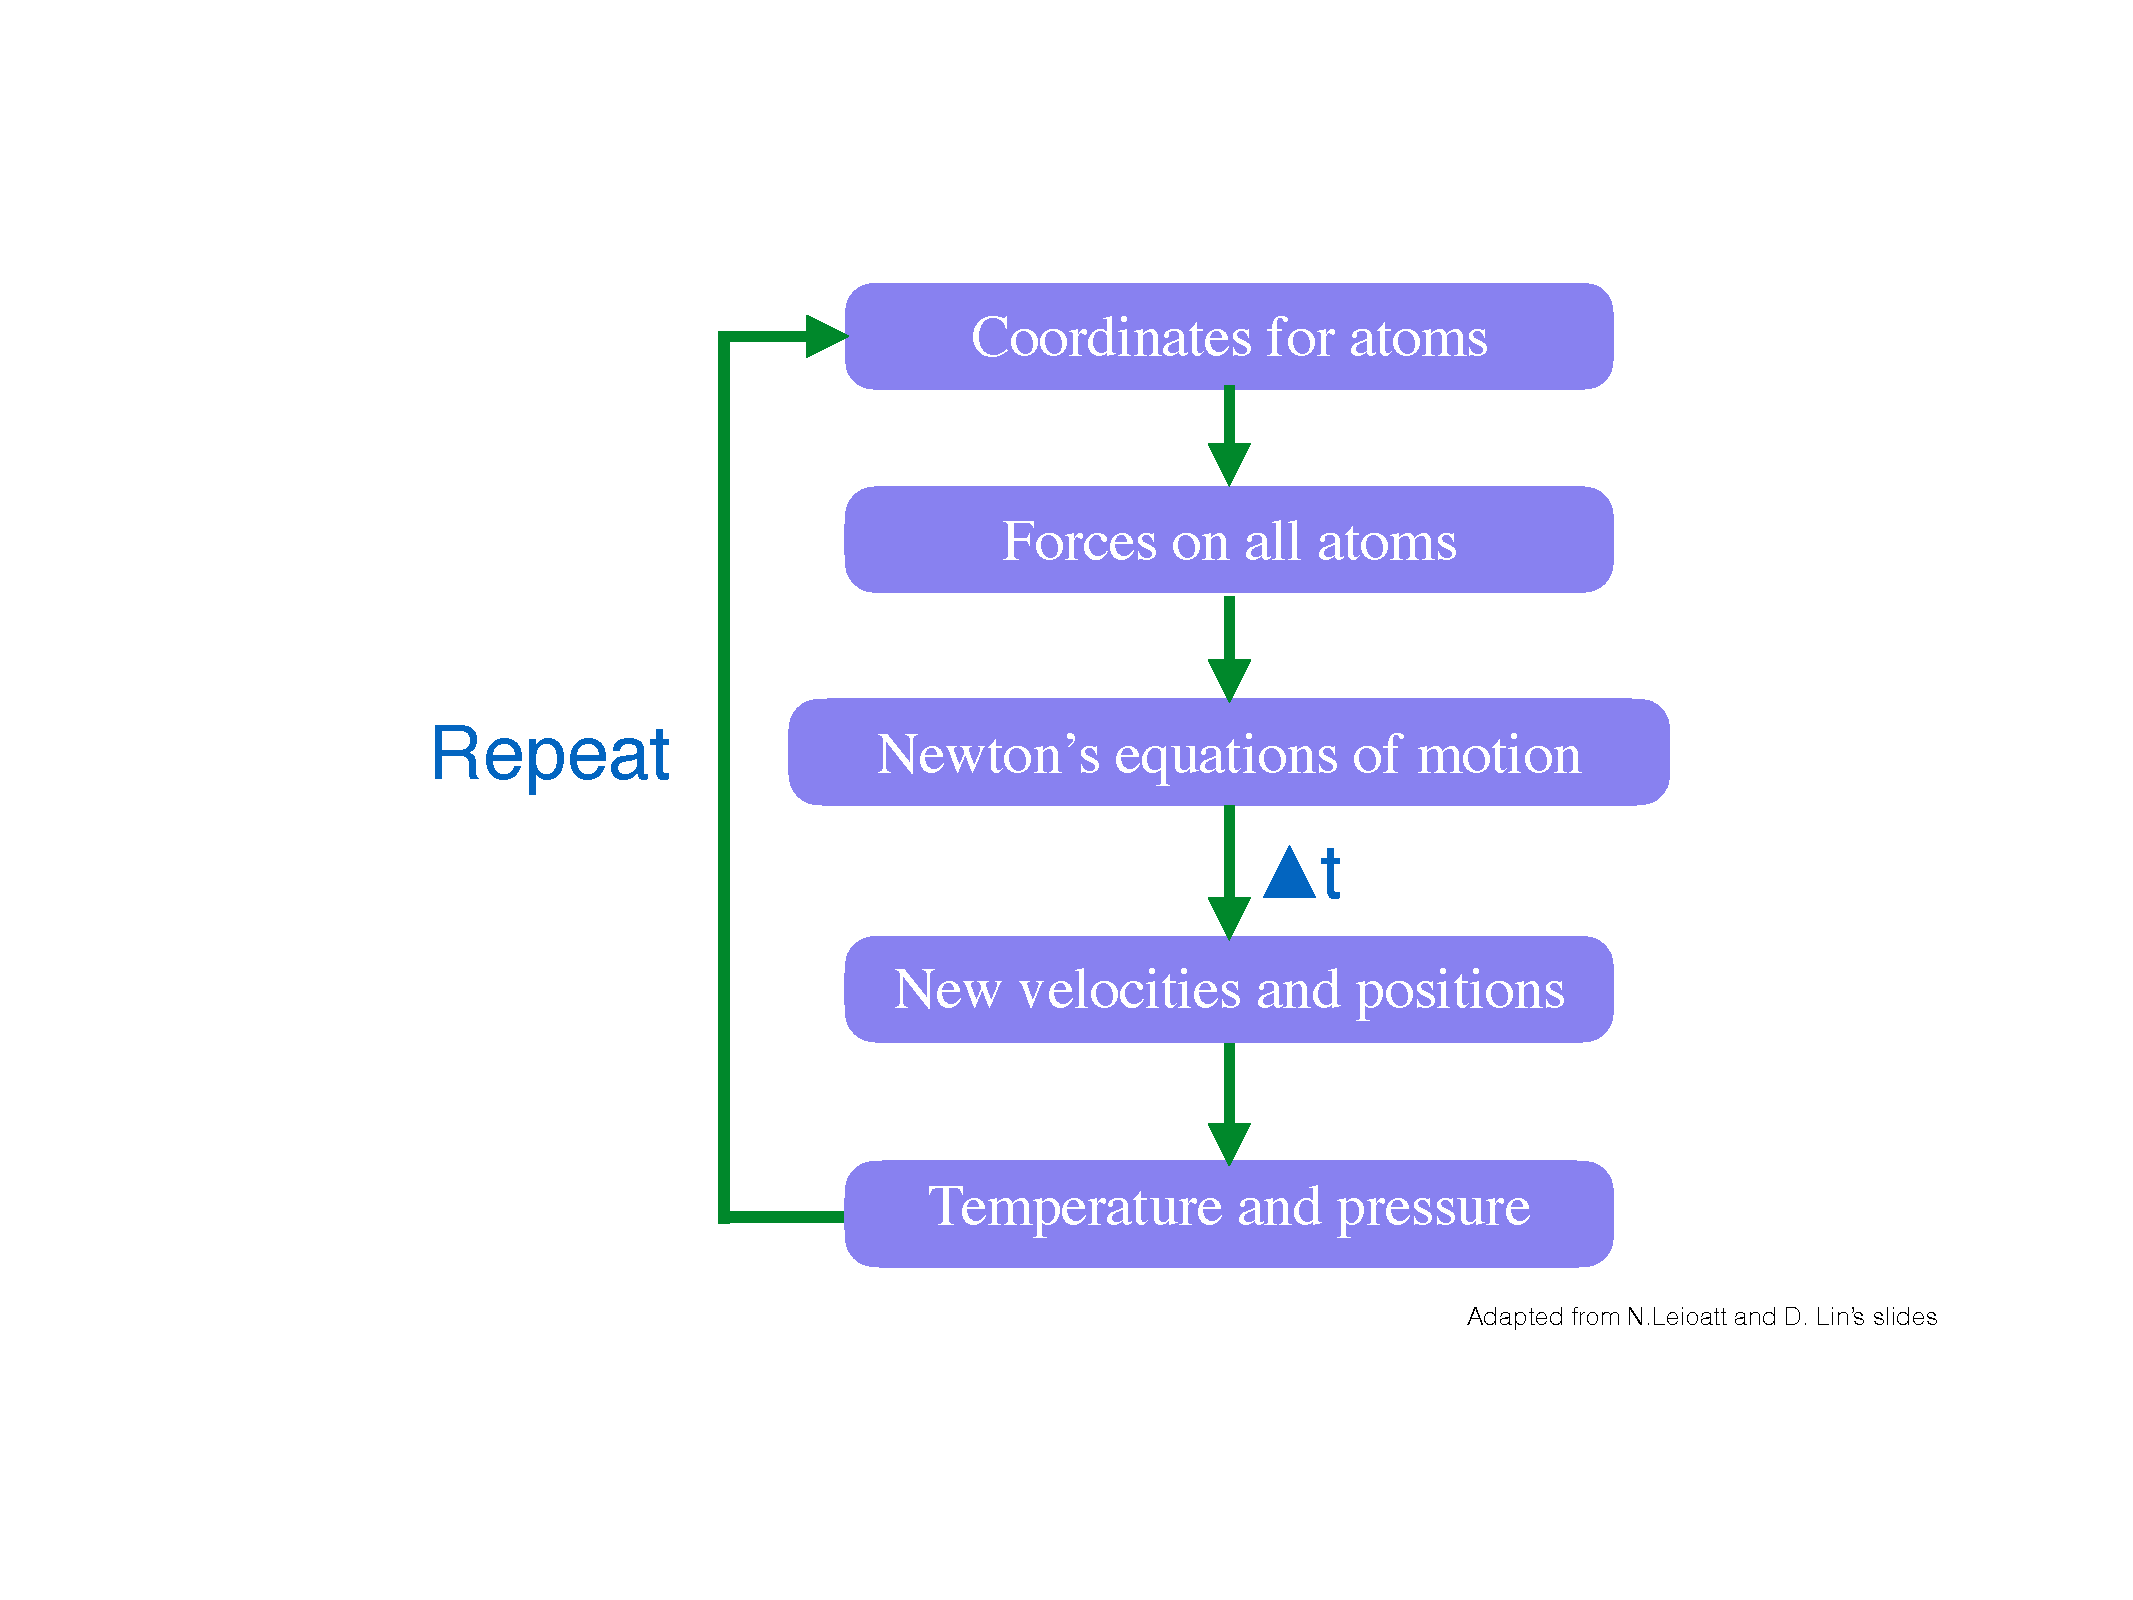
\includegraphics[width=1.0\textwidth]{chapter1_figs/md_workflow.pdf}
\caption{Workflow for molecular dynamics simulations}
\label{fig:md_wf}
\end{figure}

\section{Force fields}
\label{ss:forcefield}
Many forces act on atoms when they are part of a molecule. The balance of these physical forces make the atom stable.
Chemical molecules are bounds by bonds, bond angles and bond dihedrals. Apart from that other interactions that atoms face include electrostatic and Van der Waals. All of these forces acting on the molecules can be mathematically expressed and the information is stored as forcefield in molecular dynamics simulations. \cite{Lin2016}

\begin{equation}
\label{eq:potentials}
 U = U_{bonded} + U_{non-bonded}   
\end{equation}
where U refers to potentials associated with the bonded and non-bonded forces acting on all atoms.\cite{Lin2016}

The $U_bonded$ comprises harmonic and cosine functions defining the 
chemical bonds, angles and dihedrals respectively while non-bonded interactions are expressed in terms of coulomb's law and Lennard-Jones 
potentials.\cite{Lin2016}

\begin{equation}
\label{eq:total_bonded}
    U_{bonded} = U_{bonds} + U_{angles} + U_{dihedrals}
\end{equation}
Now the potentials associated with bonds($U_{bonds}$), angles($U_{angles}$) and dihedrals($U_{dihedrals}$) are expressed in the following equations
\begin{equation}
\label{eq:pot_bonds}
   U_{bonds}= \frac{1}{2}k_b(r_b-r_0)^2
\end{equation}
where $k_b$ is the force constant for bonds, $r_b$ is the distance between the atoms and $r_0$ is the bond distance as measured via experiments.\cite{Lin2016}
\begin{equation}
\label{eq:pot_angles}
   U_{angles}= \frac{1}{2}k_a(\theta_b-\theta_0)^2
\end{equation}
where $k_a$ is the force constant for bonds, $\theta_b$ is the angle between the three bonded atoms and $\theta_0$ is the bond angles as measured via experiments.\cite{Lin2016}
\begin{equation}
\label{eq:torsions}
    U_{torsions} = k_{\phi}\cos \left( n\phi + \phi_0 \right )
\end{equation}
where $k_{phi}$ is the multiplicative constant and $\phi$ is the angle
between two planes in which the 4 consecutive bonds are located and $\phi_0$ is the phase change.\cite{Lin2016}
 Bond and angle energies are assumed to be
harmonic potentials.
Next is the potential energy function associated with non-bonded interactions.
\begin{equation}
\label{eq:pot_nb}
    U_{non-bonded} = U_{electrostatics} + U_{vDW}
\end{equation}
These electrostatics ($U_{electrostatics}$) and van Der Waal's ($U_{vdw}$) potential energy functions can be 
expressed as follows

\begin{equation}
\label{eq:electrostatics}
    U_{electrostatics}= \frac{Q_a Q_b}{4\pi \sigma_0 r_{ab}}
\end{equation}
where $Q_{a}$ and $Q_b$ are charges associated with the atoms a and b  respectively while $r_{ab}$ is the distance between the atoms. This is done for all the atoms in the system.\cite{Lin2016}

\begin{equation}
\label{eq:vdw}
    U_{vdw} = \frac{A}{r_{ab}^{12}} - \frac{B}{r_{ab}^{6}}
\end{equation}
where $A$, $B$ are the parameters that adjusts the repulsive ($r_{ab}^{12}$)
and the attractive ($r_{ab}^6$) interactions. \cite{Lin2016}
All the parameters in the above equations can be computed through quantum 
mechanical calculations or from experimental observations. This process of 
computing parameters for different molecules is called forcefield 
parametrization.
For fengycin, I had to parametrize the ester bond that cyclizes the peptide part and the $\beta$-hydroxyl group in the acyl chain of fengycin's tail.
The correct parameters for the 
potential energy functions are important for the correct measurements
of the different physical properties of the system that we are going to calculate.\cite{Lin2016}


\section{Equations of motion}
All simulations are based on the assumption that
systems are following some of mathematical expressions where
a physical property is changing w.r.t time.
Our biological molecules and their environment are simulated 
following classical mechanics.\cite{Lin2016}
In molecular dynamics simulations we want to determine how positions
and velocities of all the atoms in the simulation box changes with time.
The Hamiltonian equations of motion which describes our system is as follows:

\begin{equation}
\label{eq:der_momentum}
\dot p = \frac{\partial H}{\partial q}
\end{equation}

\begin{equation}
\label{eq:der_positions}
\dot q = \frac{\partial H}{\partial p}
\end{equation}

where p and q represent momentum and position of all atoms and H is the Hamiltonian function. The dot
represents the derivative with respect to time.\cite{Lin2016}
The Hamiltonian function can be expressed as

\begin{equation}
    H(q,p) =  K_{p} + U_{q}
\end{equation}{}
where $K_p$ and $U_q$ are the kinetic and potential energies respectively for the system.
 
By integrating the equations \ref{eq:der_positions} and \ref{eq:der_momentum} 
we can find the positions and velocities of all atoms in the system evolving with time. 
From the individual atom positions we can derive bulk properties using statistical mechanics' concepts.
The system we consider is inside a box but if we just consider a small box comprising the system then we 
are exposing most of the atoms to surface effects. In order to avoid that
we consider the box to be periodic. Hence if an atom leaves from one side of the box it will be back on the other side of the box. These are called periodic boundary conditions.
Integration of equations  \ref{eq:der_positions} and \ref{eq:der_momentum}  are computed analytically using different algorithms and by considering that the $H(p,q)$ is measured for every $\Delta t$ timesteps usually of the order of femtoseconds.\cite{Lin2016}


\section{Temperature and Pressure control}
Simulations are usually done to get the microscopic view of the system 
because experiments have failed to have that high resolution.
But the bulk properties from experiments need to be compared with simulations.
Experiments are usually done at 298K temperature and 1atm pressure.
So we usually have an NPT ensemble.
Extended system approach is usually used to incorporate constant temperature and pressure
in molecular dynamics simulations. Here we include the thermostat and barostat's degrees of freedom 
into the Hamiltonian equations of motion. This way the position and momentum of the thermostat and barostat can modify the coordinates and velocities of the atoms in order to maintain constant temperature and pressure 
with some fluctuations. Some of the commonly used algorithms to achieve these are Nose Hoover thermostat and Parrinello-Rahman barostat. \cite{RahmanParrinello2007,Stoll1978,Brooks1995,Klein1994}

%%%%% Need to talk about general properties using Boltzman distribution
%%%%%%Time average = conformational space average

\section{Weighted Ensemble Path sampling method}
\begin{figure}
    \centering
    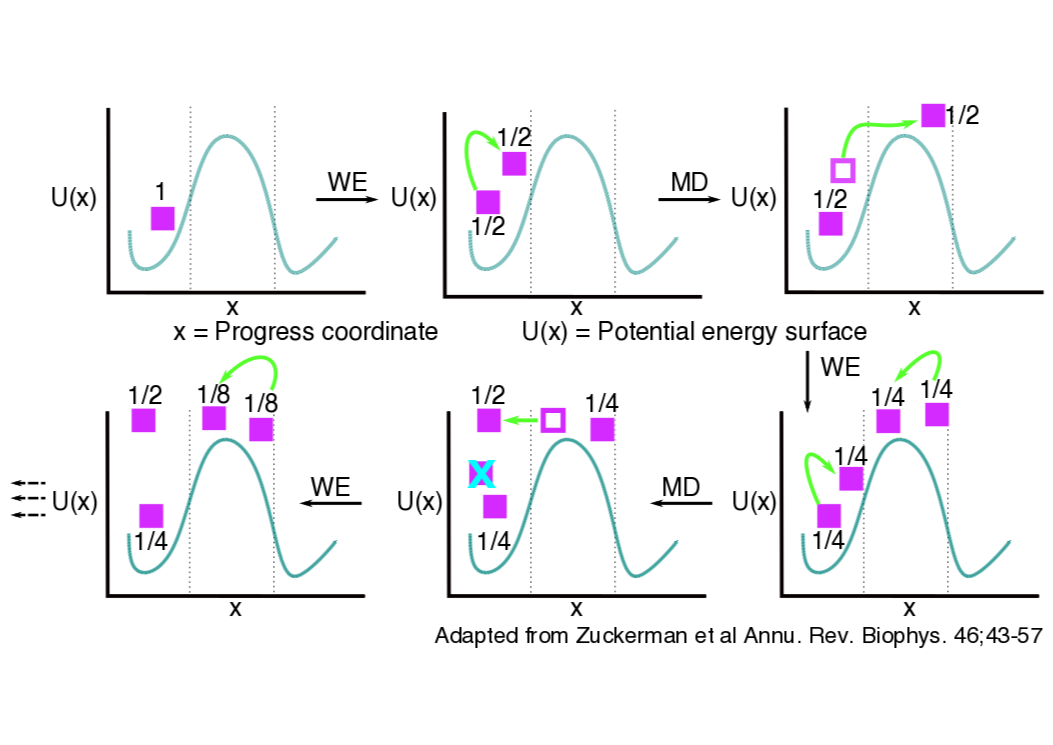
\includegraphics[width=1.0\textwidth]{chapter1_figs/we_pic.png}
    \caption{Weighted ensemble method protocol}
    \label{fig:we_fig}
\end{figure}

The numerical methods used to solve the equations \ref{eq:der_positions} and 
\ref{eq:der_momentum} are computationally expensive. In fact in order to 
simulate 20 ns long motion of \~ 40000 atoms, the GPUs in the Bluehive cluster of
University of Rochester take 24 hrs. So to compare simulations
with experiments which are measuring reactions that are hours long seem to be futile.
As technology advances, super computers are becoming more efficient. Even then if a 
ligand is bound to a protein and has residence time of minutes, traditional molecular dynamics simulations fail to estimate that long time scale.
This can be due to a high free energy barrier between bound and unbound states of the ligand or it can be insufficiency in sampling different conformation states of the
system.
Thus different algorithms have emerged that can sample states of the system which 
are usually observed at a longer time scale but are less computationally expensive.
These are called enhanced sampling methods.
In my case we used a method called weighted ensemble method. There are a variety of these enhanced sampling methods like Metadynamics, Accelerated molecular dynamics, 
Umbrella sampling and Replica exchange methods. %%%%Add the citations
But all of these methods either add additional energy to the system or 
perturb the system in some way or the other. This makes it very difficult to calculate 
kinetic properties of the system. For umbrella sampling and metadynamics methods it is 
essential to determine the slowest reaction coordinate.
This will enable us to sample state along the reaction coordinate which is the bottle neck
for the system to change from one state to another.
The protocol for weighted ensemble involves dividing the reaction coordinate into bins
as shown in Fig. %%%%Put the poster figure here%%%%
We start simulations in one of the bins. But if the system moves from one bin to another 
the trajectory is replicated. In order to maintain the total number of trajectories there is a limit to how many trajectories are there in each bin.
We also have a weight associated with each trajectory as shown in figure \ref{fig:we_fig}.%%% Fig Weighted ensemble%%%
Sum of all the weights of all the trajectories is 1.
When the trajectory is replicated the weight of the parent trajectory is split and the daughters receive 
equal parts of the parent trajectory. Thus the total weight of the trajectories 
remain 1.
If the trajectory enters a bin whose limit of number of trajectories have been reached
the trajectory is pruned but the weight of the trajectory is assigned randomly to one of the pre-existing 
trajectory in the bin.
Thus the redistribution of weights of the trajectories in different bins change 
along the progress coordinate as we iterate this process over and over.
In summary, we increase the likelihood of a system going from one bin to another by replicating the system.
This highly parallelized process helps in exploring all the conformational states of the system.
In weighted ensemble simulations no added force or energy is applied to the system
and we can customize the progress coordinate we will be using. %%%%Copy citations from the second paper

\section{Coarsed-grain Models}
\begin{figure}
    \centering
    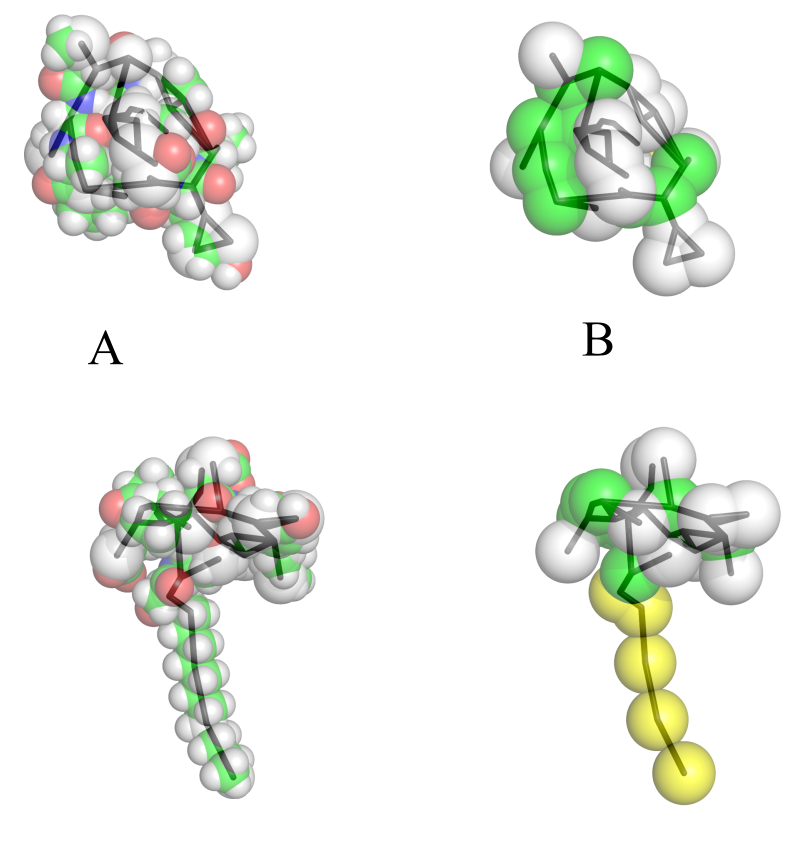
\includegraphics[width=1.0\textwidth]{chapter1_figs/structures.png}
    \caption{A: All-atom  B:Coarsed-grain representation of fengycin. Green represents carbon, white hydrogens, red oxygen and blue nitrogen. The yellow color represents the acyl tail of fengycins. \cite{Grossfield2013}}
    \label{fig:cg_feng}
\end{figure}
%%%% Put Josh'd fengycin picture %%%%
All the molecular dynamics methods described above usually considers all the atoms in the system.
This is called an all-atomistic approach. This is highly useful when we want to get
high resolution data for a particular process.
But as mentioned earlier this is computationally tedious and
the amount of simulation time obtained may not be enough to
sample a system where a change from one state to another 
takes longer time. To determine an average for a measurable physical quantity
we would need to sample the change of state A to state B multiple 
times.
Coarse-grained models are usually simplified models which involve beads which represent 
the cumulative of certain number of heavy atoms more depending on the level of 
coarse-graining required. In my case we used the MARTINI model where one bead represent 4 
heavy atoms usually. Four oxygens in waters are represented by a single bead but one ion 
atom along with its first hydration shell is represented by one bead. For cyclic chemical 
structures as in cholesterol 2 heavy atoms along with their hydrogens are represented by a 
single bead. The martini model for fengycin is shown in  Fig. %%%% Add figure
The parameters for estimating potential energies of the systems in equations 
\ref{eq:vdw},\ref{eq:electrostatics} and \ref{eq:total_bonded} was modified to incorporate 
the increased bead size. The selection of the mapping procedure (how many atoms make up a 
bead) is estimated using two factors: how much chemical properties do we want the bead to 
represent and how much reduction in degrees of freedom was obtained by coarse-graining.
Some of the areas where MARTINI has been applied till now are partitioning of lipids in 
different phases on the membrane\cite{SCHAFER2010}, formation of lipid domains on membranes\cite{Wassall2008,pastorino2012} and dimerization of membrane proteins\cite{Huber2012}. 


 \section{Setting up the problem}
Fengycin is highly specific fungicide showing no bactericidal function.\cite{Vanittanakom1986} It selectively binds to fungal cell membrane causing leakage.
As shown in the figure \ref{fig:ch2_chemical_str} fengycins are of amphiphilic nature, hence they fengycins form micelles in solution but they differ from surfactant spherical micelles due to their oblong micellar shape. Thus the fengycins micelles have the tails of fengycins bundled up and the peptide portions solvated. 
%%%%% Picture of all atom fengycins
After binding to the membrane fengycins have caused differentiation in lipid phase.
This implies different kinds lipids come together and concentrate on particular portions of the membrane. \cite{Nylander2008,Deleu2013} 
Fengycins also prefer to bind to the more liquid-like phase of the membrane which is less tightly packed than gel phase.\cite{Nylander2008}
Studies on lipid-fengycin interactions is done using vesicle leakage assays. The vesicles are spherical unilamellar lipid vesicles usually made of phospholipids and they encapsulate dyes which when released from the vesicles show fluorescence. The quantum yield associated with the fluorescence can be correlated to the rate of permeabilization. \cite{Cullis1985,FiedlerHerklotz2015}
Patel et al showed that fengycin causes membrane leakage via the all-or-none mechanism.\cite{Heerklotz2011} This implies fengycin forms large long-lived pores that causes complete efflux of the fluorescence dye instead of graded leakage which occurs when there is homogeneous short lived smaller membrane defects. \cite{Marrink2008}
Fengycin molecules partitions into the lipid as observed through cryo-EM images.\cite{Heerklotz2011}
Further fengycin addition causes aggregation of fengycins on the membrane surface as observed by Deleu et al. \cite{Nylander2008}
This leads to positive curvature of the membrane and ultimate breakage of the membrane.
Thus the selectivity of fengycin's leakage towards certain membranes can be related to the phospholipids comprising the membrane. 
In fact certain antimicrobial peptides show correlation between low miscibility in a membrane and
increase peptide association which in turn leads to better membrane leakage.\cite{huang2009}
Thus in my thesis project I have been trying to answer two broad questions.
\begin{itemize}
    \item What makes fengycin permeabilize certain membranes and not others?
    \item Does the selectivity correlated to mechanism of action of fengycins?
\end{itemize}
To answer these questions I have used molecular dynamics simulations and enhanced sampling tools. In the following section I would discuss in more detail these methods.
